\documentclass[10pt,a4paper]{article}
\usepackage[utf8]{inputenc}
\usepackage[english]{babel}
\usepackage{amsmath}
\usepackage{amsfonts}
\usepackage{amssymb}
\usepackage{graphicx}
\usepackage{indentfirst}
\usepackage{fancyvrb}
\usepackage{subfigure}
%\usepackage[hidelinks]{hyperref}
\author{Giuseppe L'Erario}
\date{}
\title{Regression}
\begin{document}
	\maketitle
	
	\section*{Introduction}
	The regression models are used for prediction problems applied on continuous data.
	
	The basic concept is the "construction" of a function able to approximate the target values given the train data (in other words, a function describing the phenomenon), in order to make a prediction upon new data.
	
	First, a \emph{Linear regression model} is analysed, then \emph{Polynomial regression models}.
	
	\section{Linear regression}
	The equation of a linear model is:
	\begin{equation}
		y = w_0 x_0 + w_1 x_1 + ... + w_n x_n = \sum w_i x_ i = w^{T} x
	\end{equation}
	where $w_0$ is the intercept of the target value axis, and $x_0=1$.
	
	When the phenomenon is described only by one variable, the model is a simple straight line:
	\begin{equation}
		y = w_0 + w_1 x
	\end{equation}
	
	After the loading of the train/test data set, I create the object \emph{PolinomialFeatures} from library \emph{sklearn} and than fit the model:
	\begin{Verbatim}
	poly=PolynomialFeatures(degree=i, include_bias=False)
	xPoly=poly.fit_transform(X_train.reshape(-1,1))
	lr=linear_model.LinearRegression()
	lr.fit(xPoly, Y_train)
	\end{Verbatim}
	
	The results are shown in fig.\ref{Interpolation}. It is clear that the phenomenon is not linear and its point cannot be interpolated by a linear function. The residuals are not concentrated around zero error line (fig.\ref{Resiuduals}) and the values of the predictione do not cover the \emph{Image} of the function\footnote{The image of the function has a range between -2 and 20, while the values of the prediction are around zero (approximately flat line).}. The \emph{mean square error} is equal to $3.83*10$.
	
	\begin{figure}%[htbp]
	\centering
	\subfigure[Interpolation\label{Interpolation}]{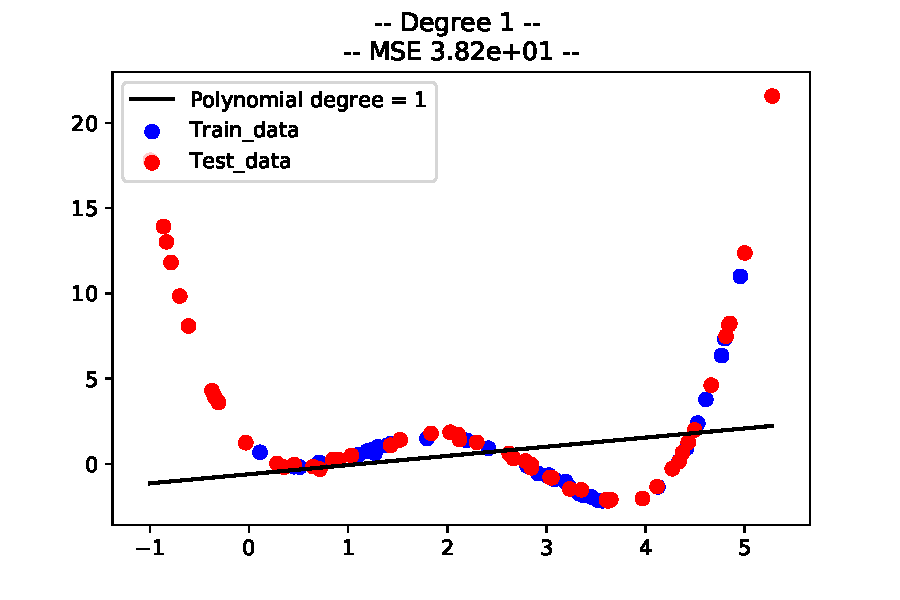
\includegraphics[width=0.8\linewidth]{../Degree1.pdf}}\qquad\qquad
	\subfigure[Residuals\label{Resiuduals}]{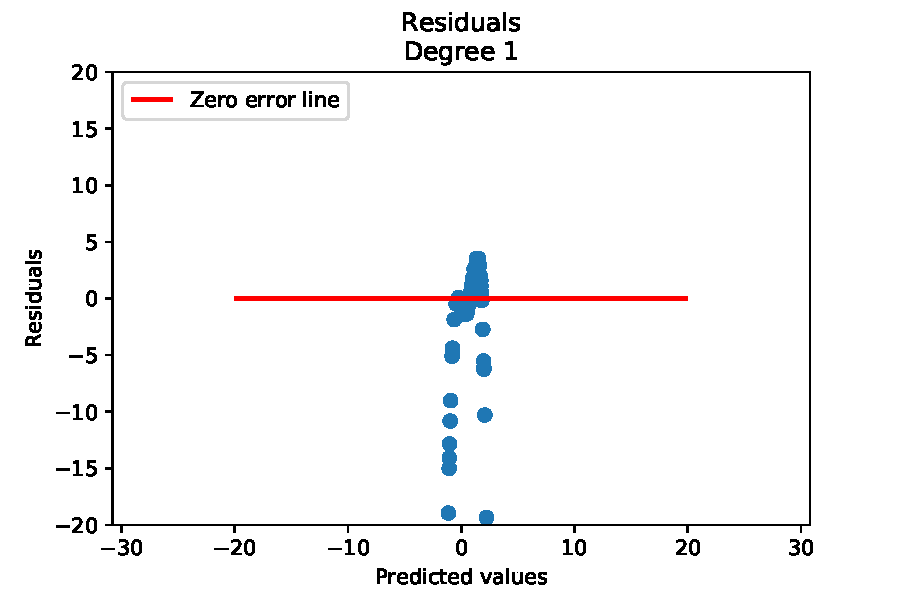
\includegraphics[width=0.8\linewidth]{../Residuals1.pdf}}
	\caption{Linear Regression\label{fig:Linear regression}}
	\end{figure}
	
	\newpage
	\section{Polynomial regression}
	With a polynomial regression the function that maps the independent variable and the value function is modelled as a polynomial of \emph{n} grade:
	\begin{equation}
		y = w_0 x^0 + w_1 x^1 + w_2 x^2 + ... + w_n x^n
	\end{equation}
	
	If the phenomenon is not linear a better prediction can be achieved with a polynomial function, taking care to find the good balance between wrong prediction and overfitting.
	
	\begin{figure}[!h]
	%\centering
	\subfigure[Degree = 2\label{Degree2}]{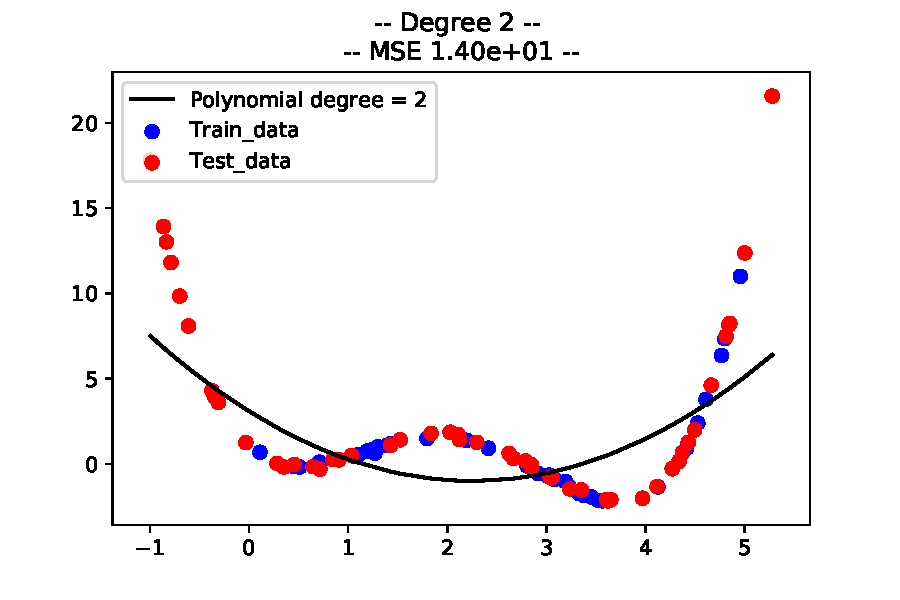
\includegraphics[width=0.4\linewidth]{../Degree2.pdf}}\qquad\qquad
	\subfigure[Degree = 3\label{Degree3}]{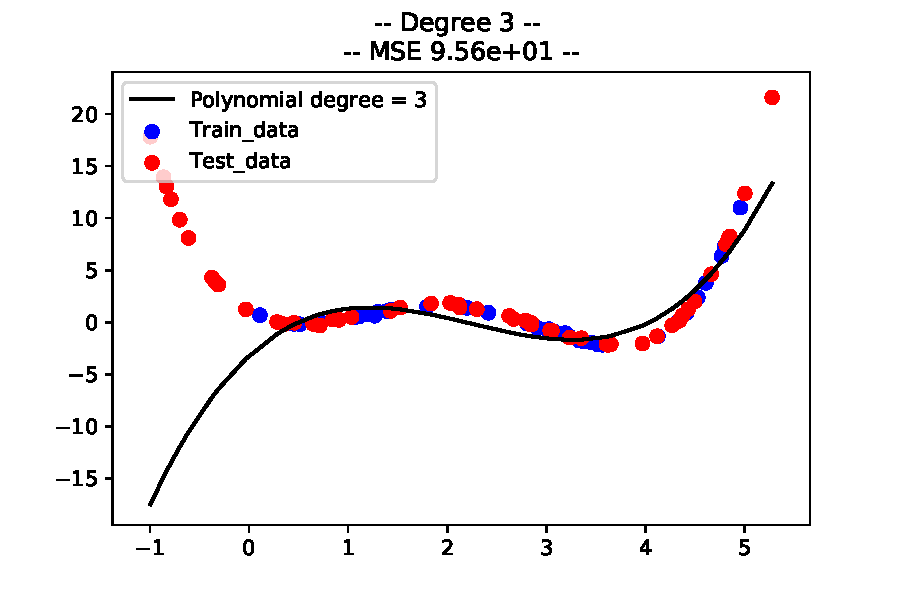
\includegraphics[width=0.4\linewidth]{../Degree3.pdf}}\qquad\qquad
	\subfigure[Degree = 4\label{Degree4}]{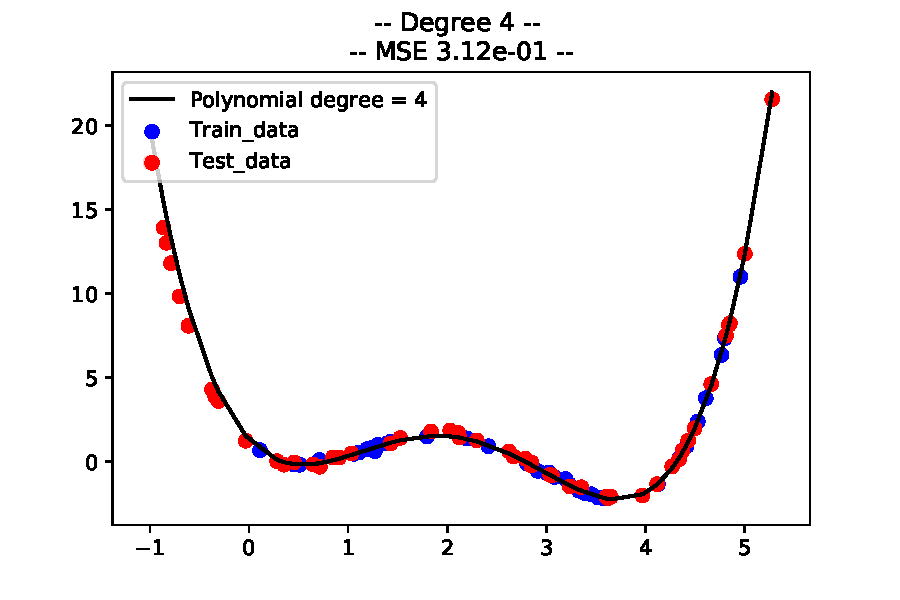
\includegraphics[width=0.4\linewidth]{../Degree4.pdf}}\qquad\qquad
	\subfigure[Degree = 5\label{Degree5}]{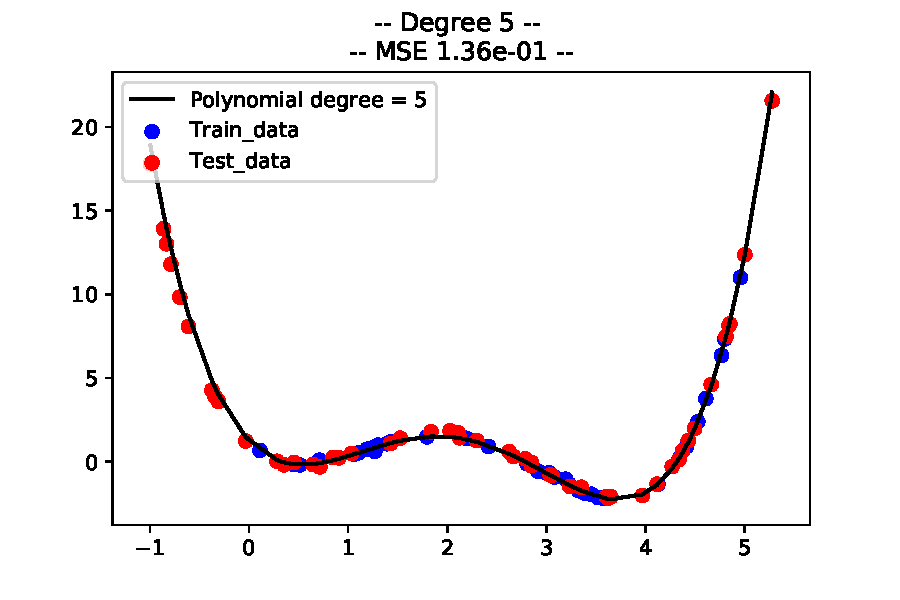
\includegraphics[width=0.4\linewidth]{../Degree5.pdf}}\qquad\qquad
	\subfigure[Degree = 6\label{Degree6}]{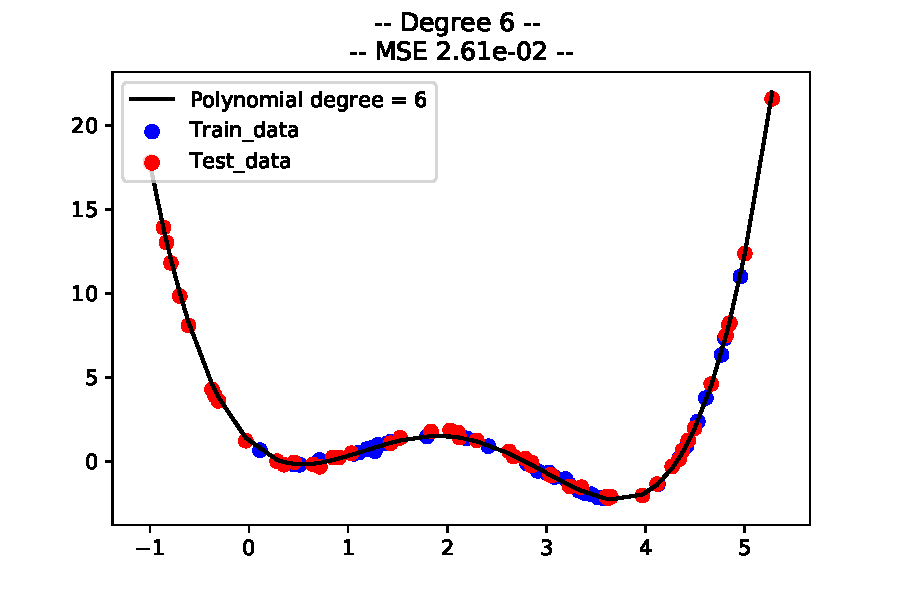
\includegraphics[width=0.4\linewidth]{../Degree6.pdf}}\qquad\qquad
	\subfigure[Degree = 7\label{Degree7}]{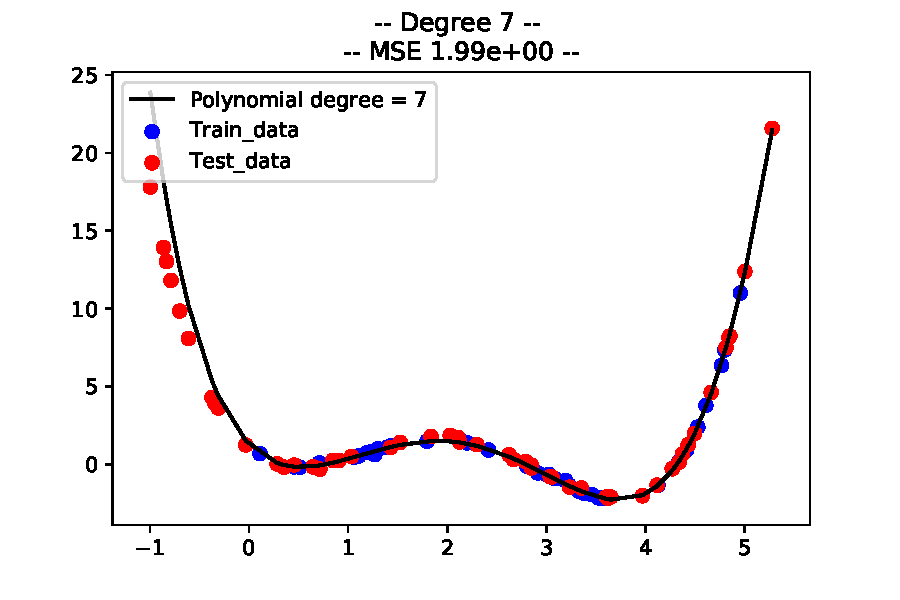
\includegraphics[width=0.4\linewidth]{../Degree7.pdf}}\qquad\qquad
	\subfigure[Degree = 8\label{Degree8}]{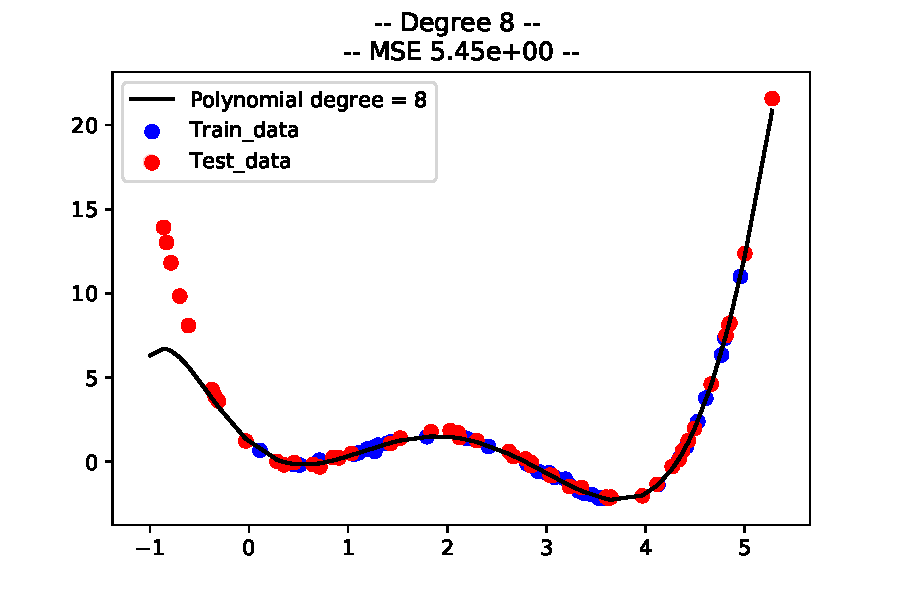
\includegraphics[width=0.4\linewidth]{../Degree8.pdf}}\qquad\qquad
	\subfigure[Degree = 9\label{Degree9}]{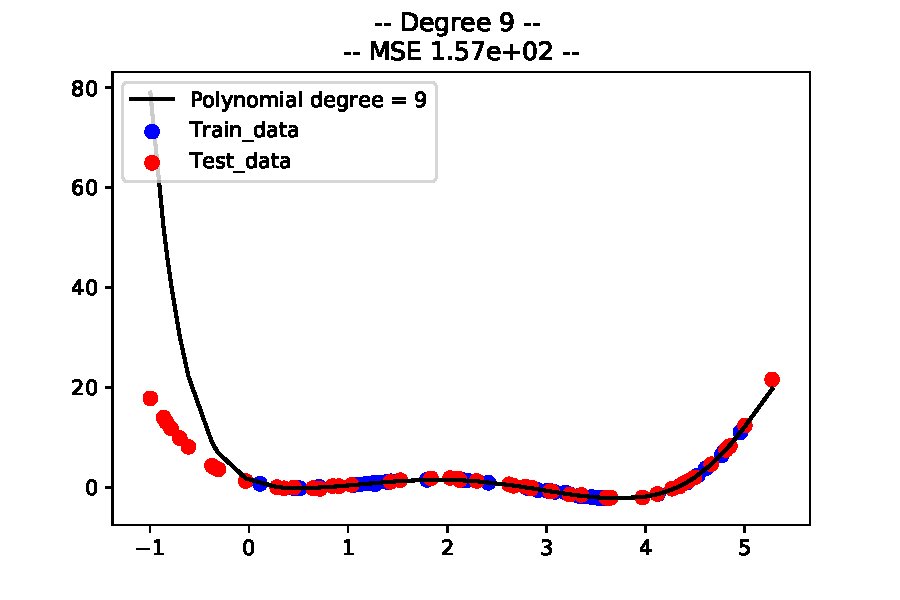
\includegraphics[width=0.4\linewidth]{../Degree9.pdf}}\qquad\qquad
	\caption{Polynomial Regression\label{Polyreg}}
	\end{figure}
	
	The \emph{Mean Square Error} is plotted in fig.\ref{fig:MeanSquareError}.
	
	\begin{figure}[!h]
	\centering
	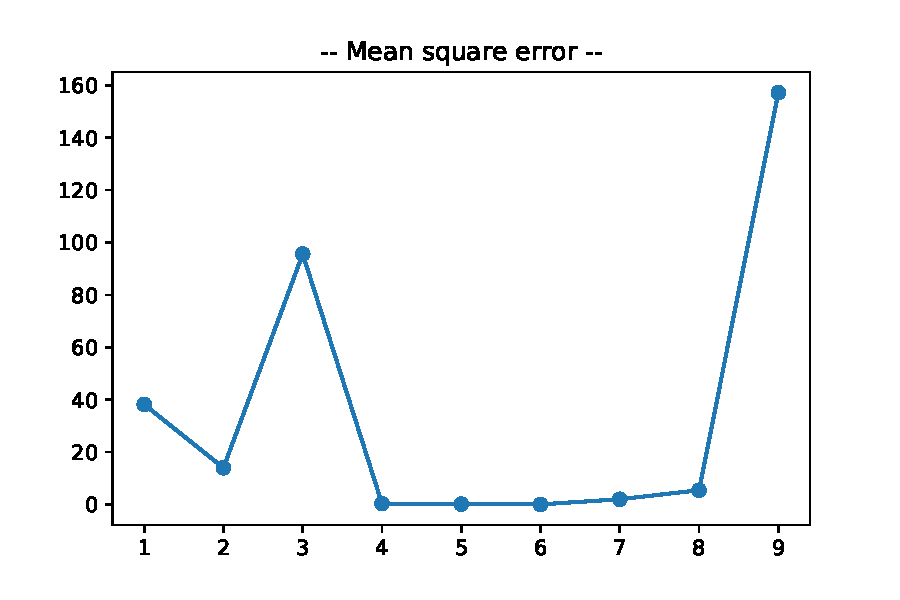
\includegraphics[width=0.7\linewidth]{../MeanSquareError}
	\caption{Mean square error}
	\label{fig:MeanSquareError}
	\end{figure}
	
	
	The lowest error is reached with $6^{th}$ degree polynomial, in fig.\ref{Degree6}, with a $MSE=2.608*10^{-2}$. We can observe a similar behaviour in polynomials from degree 4 to 8. 
	
	The $9^{th}$ degree polynomial (fig.\ref{Degree9}) presents a sensible overfitting, while the $3^{rd}$ degree polynomial (fig.\ref{Degree3}) has a great error because of its shape. 
	
	\begin{figure}[!h]
		\centering
		\subfigure[Degree = 3\label{Residuals3}]{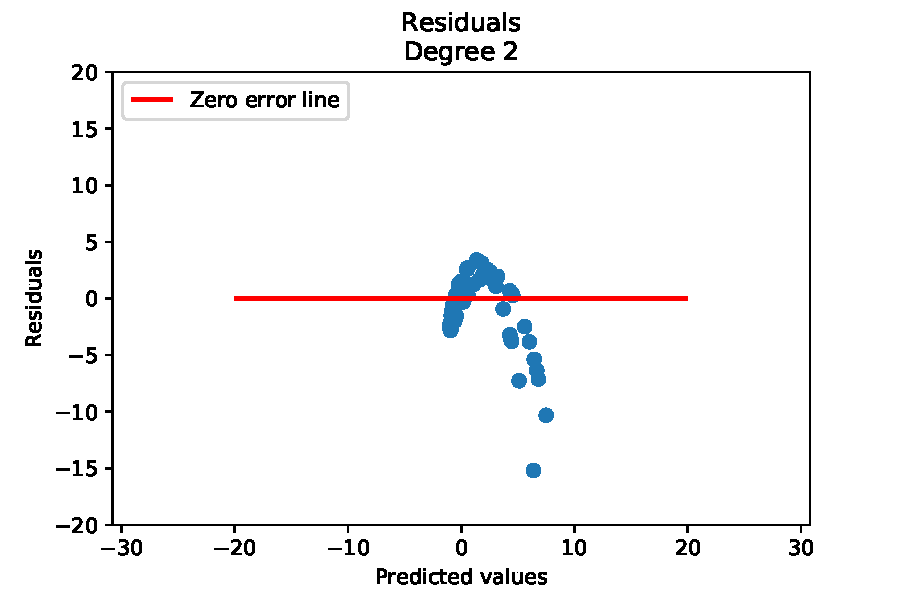
\includegraphics[width=0.4\linewidth]{../Residuals2.pdf}}\qquad\qquad
		\subfigure[Degree = 6\label{Residuals6}]{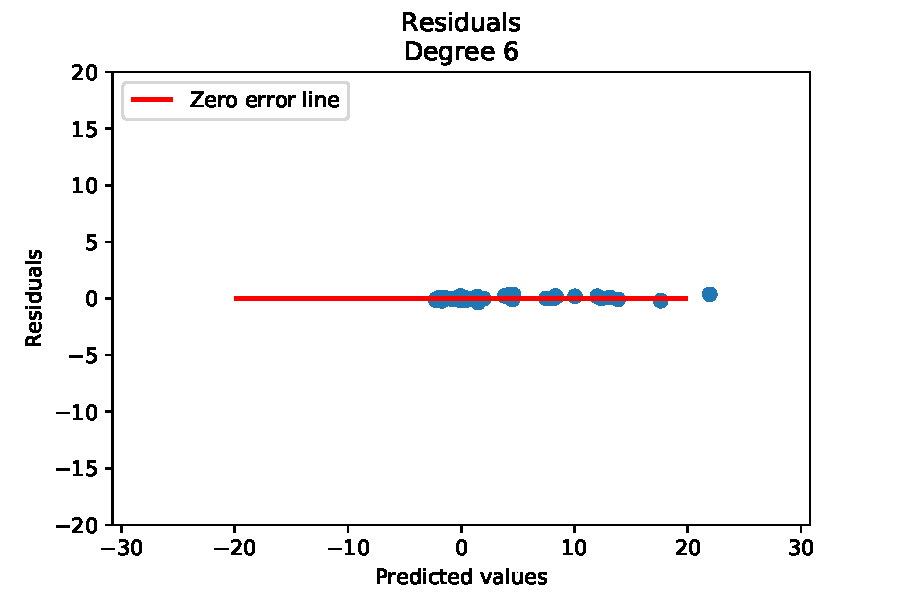
\includegraphics[width=0.4\linewidth]{../Residuals6.pdf}}\qquad\qquad
		\subfigure[Degree = 9\label{Residuals9}]{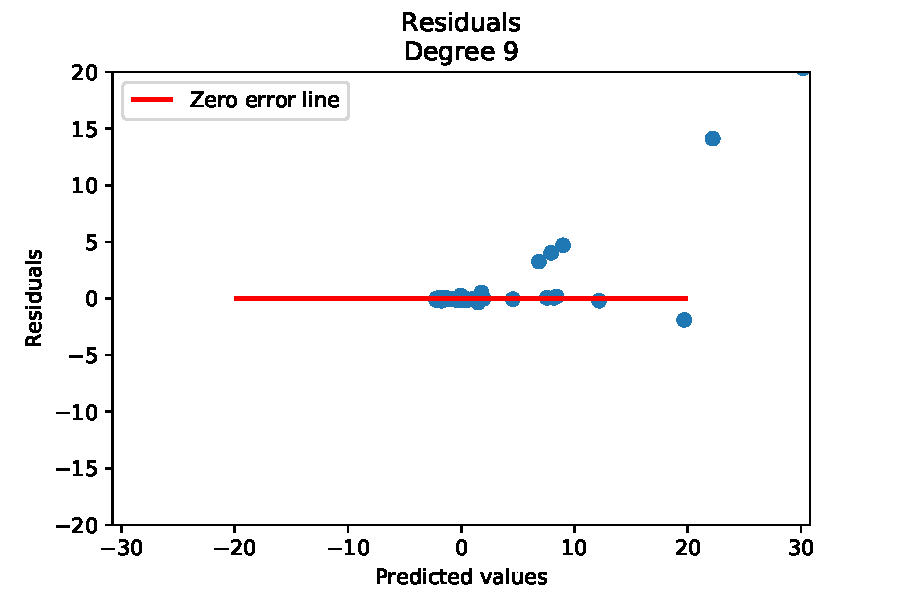
\includegraphics[width=0.4\linewidth]{../Residuals9.pdf}}\qquad\qquad
		\caption{Residuals of $3^{rd},6^{th}, 9^{th}$ degree polynomials \label{Residuals__}}
	\end{figure}
	
	The gap between the test values and the prediction values is presented in fig.\ref{Residuals__}: the values in fig.\ref{Residuals6} are all around zero line error, confirming that $6^{th}$ degree polynomial regression leads to the best performances. 
	

\end{document}